% article example for classicthesis.sty
\documentclass[10pt,a4paper]{article} % KOMA-Script article scrartcl
\usepackage{lipsum}
\usepackage{graphicx}
\usepackage{url}
\usepackage[nochapters]{classicthesis}

\usepackage{listings}
\lstset{
    language=Python,
    basicstyle=\ttfamily\small,
    aboveskip={1.0\baselineskip},
    belowskip={1.0\baselineskip},
    columns=fixed,
    extendedchars=true,
    breaklines=true,
    tabsize=4,
    prebreak=\raisebox{0ex}[0ex][0ex]{\ensuremath{\hookleftarrow}},
    frame=lines,
    showtabs=false,
    showspaces=false,
    showstringspaces=false,
    keywordstyle=\color[rgb]{0.627,0.126,0.941},
    commentstyle=\color[rgb]{0.133,0.545,0.133},
    stringstyle=\color[rgb]{01,0,0},
    numbers=left,
    numberstyle=\small,
    stepnumber=1,
    numbersep=10pt,
    captionpos=t,
    escapeinside={\%*}{*)}
}


\begin{document}
    \title{Trabajo Especial I}
    \author{Carlos Mart\'in Becerra}
    \date{\today} % no date
    
    \maketitle
    
    \tableofcontents
    
    \newpage
    \section{Introducci\'on}
    \subsection{Descripci\'on del problema}
    Un lavadero de ropa autom\'atico cuenta con 5 m\'aquinas en servicio en funcionamiento constante. Como las m\'aquinas lavadoras se rompen peri\'odicamente, el lugar cuenta 2 m\'aquinas de repuesto, todas ellas id\'enticas entre s\'i. A su vez el lavadero cuenta con el servicio t\'ecnico de reparaci\'on provisto por un solo operario. El mismo solo puede arreglar una m\'aquina a la vez.\\
    Este sistema fallar\'a en el momento que no se encuentren 5 m\'aquinas en funcionamiento, o equivalentemente, que el t\'ecnico deba arreglar m\'as de dos m\'aquinas.\\
    Teniendo en cuenta todo esta informaci\'on, el due\~no del lavadero desea determinar los siguientes puntos:

    \begin{itemize}
    \item El tiempo promedio que transcurre hasta que el lavadero deja de ser operativo, es decir, que falla el sistema.
    \item Si tiempo promedio que transcurre hasta que el lavadero falla mejora agregando un t\'ecnico u otra m\'aquina de repuesto.
    \end{itemize}
    
    Para ello simularemos un modelo de reparaci\'on. Los tiempos de funcionamiento de las m\'aquinas hasta descomponerse est\'an determinados con respecto a una variable aleatoria de distribuci\'on exponencial con un tiempo medio hasta fallar de $T_f$, y que tiempo que les lleva a las m\'aquinas ser reparadas por el t\'ecnico es determinado por una variable aleatoria exponencial con tiempo medio igual a $T_r$, estas variables son independientes entre s\'i.
    
    \newpage
    \section{Algoritmo}
    \subsection{Descripci\'on de las variables}
    Previamente a describir el algoritmo empleado para simular el sistema, introduciremos las variables que ser\'an utilizadas en el mismo:
    \begin{itemize}
    \item $t$ : Ser\'a la variable de tiempo.
    \item $r$ : Describir\'a la cantidad de m\'aquinas rotas en el instante t.
    \item $S$ : Es la cantidad de m\'aquinas de repuesto, que a su vez es m\'axima cantidad de m\'aquinas que podr\'ian estar averiadas al mismo tiempo.
    \item $eventos$ : Una lista de tiempos que describe los momentos en los cuales fallar\'an las m\'aquinas
    \item $t^{\star}$ : Especifica el tiempo en que terminar\'a de reparar una m\'aquina el t\'ecnico. En caso de que el operario no se encuentre trabajando, se definir\'a como infinito.
    \item $T_f$ : Tiempo de falla de una m\'aquina del sistema.
    \item $T_r$ : Tiempo medio de reparaci\'on de las m\'aquinas.
    \end{itemize}

    \subsection{Algoritmo}
    En el siguiente pseudo-c\'odigo se muestra como se realiza la simulaci\'on de un modelo de reparaci\'on hasta que el mismo falla.
    
    \begin{lstlisting}[caption=Funciones auxiliares.]
init()
while True:
    if (events[0] < %*$t^{\star}$*)):
        t = events[0]
        r = r + 1
        if (r == S+1):
            return t;
        else:
            x = exponencial(%*$T_f$*))
            events[0] = t + x
            events.sort()
            if (%*$t^{\star}$*) == %*$\infty$*)):
                %*$t^{\star}$*) = t + exponencial(%*$T_r$*))
    else: 
        t = %*$t^{\star}$*)_
        r = r - 1
        if (r > 0):
            %*$t^{\star}$*) = t + exponencial(%*$T_r$*))
        else:
            %*$t^{\star}$*) = %*$\infty$*)
    \end{lstlisting}
Las funciones auxiliares init y exponencial\footnote{La forma en la que est\'a definida la funcion auxiliar para crear variables aleatorias con distribuci\'on exponencial permite evitar tener tomar como argumento 1 sobre la media.} son definidas a continuaci\'on\footnote{Notar que todas las variables utilizadas est\'an definidas globalmente.}:
    \begin{lstlisting}[caption=Pseudo-c\'odigo del las funciones auxiliares.]
def init():
    t = r = 0; %*$t^{\star}$*) = %*$\infty$*)
    exponencial = (lambda x: -log(Uniforme()) * x)
    events = [exponencial(%*$T_f$*)) for _ in range(N)]
    events.sort()
    \end{lstlisting}
    
    \newpage
    \section{Resultados}
    En primer lugar analizaremos el funcionamiento del sistema inicial, para luego hacer una comparaci\'on del funcionamiento del mismo cuando se agrega un operario y cuando se agrega una m\'aquina de repuesto. Esto nos permitir\'a llegar a una conclusi\'on fundamentada sobre que es lo m\'as conveniente para el due\~no del lavadero al momento de tomar una decisi\'on.
    
    \subsection{Sistema con un t\'ecnico y dos repuestos}
    A continuaci\'on se muestra un histograma con los valores de 10000 simulaciones de tiempos de fallo del sistema funcionando con 2 m\'aquinas de repuesto y 1 solo operario.
    \begin {figure}[!htb]
    \centering
    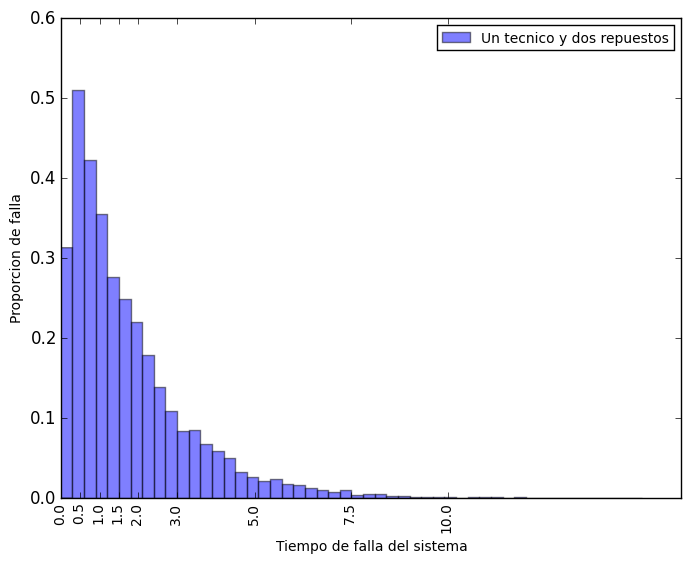
\includegraphics[width=12cm] {img/1op2rep}
    \end {figure}
    
    El gr\'afico hace evidente que lo m\'as probable es que el sistema falle entre el primer y segundo mes de funcionamiento. Tambi\'en se complementa al gr\'afico la siguiente tabla con los resultados del tiempo promedio de falla y la variaci\'on del mismo luego de haber realiado 100, 1000 y 10000 iteraciones.
    
    \begin{center}
        \begin{tabular}{ c| c| c}
            Iteraciones & Esperanza & Desv\'io est\'andar \\ \hline
            100&    1.84916 & 1.67891 \\ \hline
            1000&   1.74255 & 1.57913 \\ \hline
            10000&  1.74317 & 1.60938 \\ \hline
        \end{tabular}
    \end{center}
    
    La modificaci\'on del algoritmo original utilizado para realizar esta simulaci\'on puede encontrarse en el apendice.
    
    \subsection{Sistema con un t\'ecnico y tres repuestos}
    A continuaci\'on se muestra un histograma con los valores de 10000 simulaciones de tiempos de fallo del sistema funcionando con 3 m\'aquinas de repuesto y 1 solo operario.
    \begin {figure}[!htb]
    \centering
    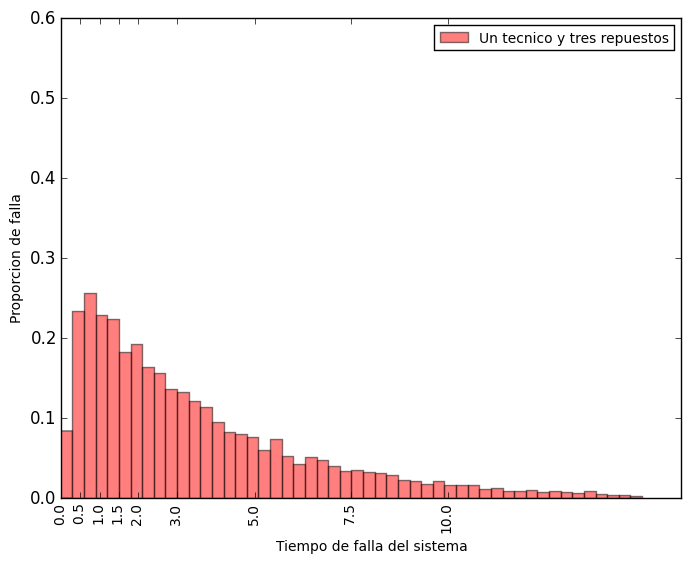
\includegraphics[width=12cm] {img/1op3rep}
    \end {figure}

    Ahora con la incorporaci\'on de otra m\'aquina lavadora que puede ser utilizada como repuesto, podemos ver que la periodicidad con la cual falla el sistema ahora se encuentra m\'as distribuida, haciendo as\'i que sea m\'as probable que el sistema pueda funcionar durante m\'as tiempo. El gr\'afico muestra que hay m\'as posibilidades de que el sistema dure m\'as de un mes en funcionamiento. \\
    Se complementa al gr\'afico la siguiente tabla con los resultados del tiempo promedio de falla y la variaci\'on del mismo luego de haber realizado 100, 1000 y 10000 iteraciones.
    
    \begin{center}
        \begin{tabular}{ c| c| c}
            Iteraciones & Esperanza & Desv\'io est\'andar \\ \hline
            100&    3.33427 & 3.22612  \\ \hline
            1000&   3.22161 & 3.30346  \\ \hline
	        10000&  3.57698 & 3.27928  \\ \hline

        \end{tabular}
    \end{center}
    
    \subsection{Sistema con dos t\'ecnicos y dos repuestos}
    A continuaci\'on se muestra un histograma con los valores de 10000 simulaciones de tiempos de fallo del sistema funcionando con 2 m\'aquinas de repuesto y 2 operarios.
    \begin {figure}[!htb]
    \centering
    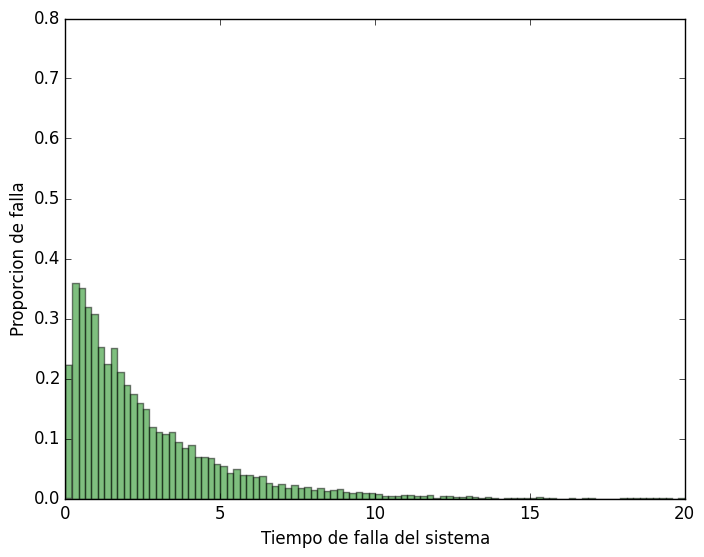
\includegraphics[width=12cm] {img/2op2rep}
    \end {figure}

    En el caso de incorporar la participaci\'on de otro t\'ecnico de reparaci\'on al sistema, se puede notar que hay cierta similitud a cuando solo tenemos un solo operario, ya que sigue habiendo lo m\'as probables es que el sistema falle dentro de los primeros dos meses, solo que ahora esta probabilidad se ha dilatado en los meses que contin\'uan. Haciendo as\'i que el sistema llegue a durar m\'as. \\
    Se complementa al gr\'afico la siguiente tabla con los resultados del tiempo promedio de falla y la variaci\'on del mismo luego de haber realizado 100, 1000 y 10000 iteraciones.
    
    \begin{center}
        \begin{tabular}{ c| c| c}
            Iteraciones & Esperanza & Desv\'io est\'andar \\ \hline
            100&    2.36958 & 2.56351  \\ \hline
            1000&   2.75588 & 2.44585  \\ \hline
            10000&  2.58391 & 2.41951  \\ \hline
        \end{tabular}
    \end{center}

    \newpage
    \section{Conclusi\'on}
    Finalmente luego de haber realizado la simulaci\'on del sistema en su estado actual y luego de realizar cada cambio posible podemos llegar a una conclusi\'on verificada sobre que es lo m\'as propicio para el due\~no del lavadero. \\
    
    \begin {figure}[!htb]
    \centering
    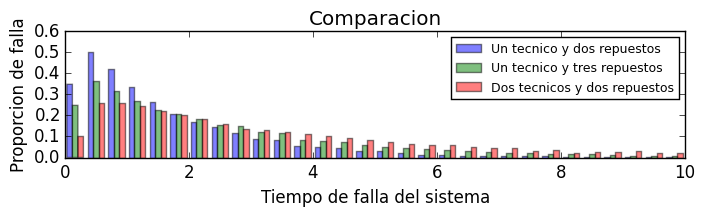
\includegraphics[width=12cm] {img/comparisson}
    \end {figure}
    
    El histograma con los valores de 10000 simulaciones comparando los tiempos de fallo del sistema en las diferentes situaciones planteadas.\\ 
    Gracias a este gr\'afico y las an\'alisis antes realizados, es m\'as f\'acil llegar a la conclusi\'on de que, en el caso de ambas mejoras al sistema tengan el mismo costo, es preferible adquirir un otra m\'aquina lavadora de repuesto.

    \newpage
    \section{Ap\'endice}
    \subsection{Algoritmo para la simulaci\'on con dos operarios}
    El siguiente algoritmo representa una simulaci\'on del sistema empleando el trabajo de 2 t\'ecnicos.\\
    Las funciones auxiliares init y exponencial son las mismas definidas para el primer algoritmo:

    \begin{lstlisting}[caption=Funciones auxiliares.]
init()
while True:
        if (events[0] < %*$t^{\star}_1$*) and events[0] < %*$t^{\star}_2$*)):
            t = events[0]
            r = r + 1
            if (r == S+1):
                return t;
            else:
                events[0] = t + exponencial(%*$T_f$*))
                events.sort()
                if (%*$t^{\star}_1$*) == %*$\infty$*)):
                    %*$t^{\star}_1$*) = t + exponencial(%*$T_r$*))
                    continue
                if (%*$t^{\star}_2$*) == %*$\infty$*)):
                    %*$t^{\star}_2$*) = t + exponencial(%*$T_r$*))

        elif (events[0] >= %*$t^{\star}_1$*)):
            t = %*$t^{\star}_1$*)
            r = r - 1
            if ((r > 1 and %*$t^{\star}_2$*) != %*$\infty$*)) or (%*$t^{\star}_2$*) == %*$\infty$*) and r > 0)):
                %*$t^{\star}_1$*) = t + exponencial(%*$T_r$*))
            else:
                %*$t^{\star}_1$*) = %*$\infty$*)

        elif (events[0] >= %*$t^{\star}_2$*)):
            t = %*$t^{\star}_2$*)
            r = r - 1
            if ((r > 1 and %*$t^{\star}_1$*) != %*$\infty$*)) or (%*$t^{\star}_1$*) == %*$\infty$*) and r > 0)):
                %*$t^{\star}_2$*) = t + exponencial(%*$T_r$*))
            else: 
                %*$t^{\star}_2$*) = %*$\infty$*)
    \end{lstlisting}
\end{document}
